%****************************************************************************%
%* DIET User's Manual deploying chapter file                                *%
%*                                                                          *%
%*  Author(s):                                                              *%
%*    - Holly DAIL (Holly.Dail@ens-lyon.fr)                                 *%
%*    - Raphael BOLZE (Raphael.Bolze@ens-lyon.fr)                           *%
%*    - Eddy CARON (Eddy Caron@ens-lyon.fr)                                 *%
%*    - Philippe COMBES (Philippe.Combes@ens-lyon.fr)                       *%
%*    - Benjamin DEPARDON (Benjamin.Depardon@ens-lyon.fr)                   *%
%*                                                                          *%
%* $LICENSE$                                                                *%
%****************************************************************************%
%* $Id: deploy.tex,v 1.27 2011/05/02 10:01:43 bdepardo Exp $
%* $Log: deploy.tex,v $
%* Revision 1.27  2011/05/02 10:01:43  bdepardo
%* Corrected a few typos.
%* Renamed "round-robin" scheduler into "least recently used" scheduler as this
%* is closer to the behavior of this scheduler.
%*
%* Revision 1.26  2010/09/19 10:35:46  bdepardo
%* Added a section on how to choose the shape of the hierarchy
%*
%* Revision 1.25  2010/03/29 21:18:17  ecaron
%* Update GoDIET commands
%*
%* Revision 1.24  2010/02/25 08:05:27  ycaniou
%* e.g -> Use macro
%* Typo + ispell
%*
%* Revision 1.23  2010/02/25 06:45:38  ycaniou
%* Add local variables
%*
%* Revision 1.22  2010/01/21 14:05:58  bdepardo
%* DIET -> \diet
%* SeD -> \sed
%* GoDIET -> \godiet
%*
%* Revision 1.21  2008/07/16 23:02:48  ecaron
%* Fixe the problem with too long list of hosts
%*
%* Revision 1.20  2008/03/04 16:12:37  bdepardo
%* Added a link to the file examples/commented.xml for GoDIET.
%*
%* Revision 1.19  2006/11/29 16:55:49  dloureir
%* minor corrections
%*
%* Revision 1.18  2006/05/12 12:12:32  sdahan
%* Add some documentation about multi-MA
%*
%* Bug fix:
%*  - segfault when the neighbours configuration line was empty
%*  - deadlock when a MA create a link on itself
%*
%* Revision 1.17  2005/07/13 07:56:15  hdail
%* Corrected error in xml example and added console instructions to GoDIET section.
%*
%* Revision 1.16  2005/07/12 21:44:28  hdail
%* - Correcting small problems throughout
%* - Modified deployment chapter to have a real section for deploying via GoDIET
%* - Adding short xml example without the comments to make a figure in GoDIET
%*   section.
%*
%* Revision 1.15  2005/06/28 15:53:02  hdail
%* Completed corrections for config file examples and text explaining launch of
%* each component.
%*
%* Revision 1.14  2005/06/28 13:57:55  hdail
%* Described GoDIET and updating section on launching by hand.
%*
%* Revision 1.13  2005/06/24 14:27:07  hdail
%* Correcting english problems & updating descriptions that are no longer true.
%*
%* Revision 1.12  2005/06/14 08:26:32  ecaron
%* Deployment section should introduce GoDIET (Fixme for Holly)
%*
%* Revision 1.11  2005/05/29 13:51:22  ycaniou
%* Moved the section concerning FAST from description to a new chapter about FAST
%* and performances prediction.
%* Moved the section about convertors in the FAST chapter.
%* Modified the small introduction in chapter 1.
%* The rest of the changes are purely in the format of .tex files.
%*
%* Revision 1.10  2004/10/25 08:59:56  sdahan
%* add the multi-MA documentation
%*
%* Revision 1.9  2004/09/28 07:03:39  rbolze
%* remove useAsyncAPI parameter
%*
%* Revision 1.8  2004/07/12 08:33:58  rbolze
%* explain how to copy cfgs file in install_dir/etc directory and correct my english
%****************************************************************************%

\newcommand{\bla}{}
\chapter{Deploying a \diet platform}
\label{ch:deploying}


Deployment is the process of launching a \diet platform including agents and
servers. For \diet, this process includes writing configuration files for each
element and launching the elements in the correct hierarchical order. There are
three primary ways to deploy \diet.

Launching \textbf{by hand} is a reasonable way to deploy \diet for small-scale
testing and verification. This chapter explains the necessary services, how to
write \diet configuration files, and in what order \diet elements should be
launched. See Section~\ref{sec:deployBasics} for details.

Using \textbf{\godiet}, a Java-based tool for automatic \diet deployment that
manages the creation of configuration file, the staging of files, the launch of elements,
the monitoring and reporting upon successful launch, and the cleanup process when the \diet
deployment is no longer needed. See Section~\ref{sec:deployGoDIET} for
details.

\textbf{Writing your own scripts} is a surprisingly popular approach. This
approach often looks easy initially, but can sometimes take much, much longer
than expected, as there are many complexities to manage. Learn how to use \godiet -- it
will save you time!




\section{\godiet}
\label{sec:deployGoDIET}

%%Description
\godiet is a cross-platform tool that helps you automate ad-hoc deployment and
management procedures for a \diet platform. It manages
the creation of configuration files, the staging of files, the launch of software components, the monitoring and the reporting. \godiet is extremely useful for large deployments on a complex physical infrastructure. The main features are:
\begin{itemize}
  \item \bla Complete running application customization. Infrastructure agnostic approach;
  \item command-line interface;
  \item distributed command execution via SSH;
  \item real-time monitoring of applications' states;
  \item handling of complex physical infrastructure, with firewalls and multiple local- and wide-area networks.
\end{itemize}
\begin{figure}[h]
  \centering
  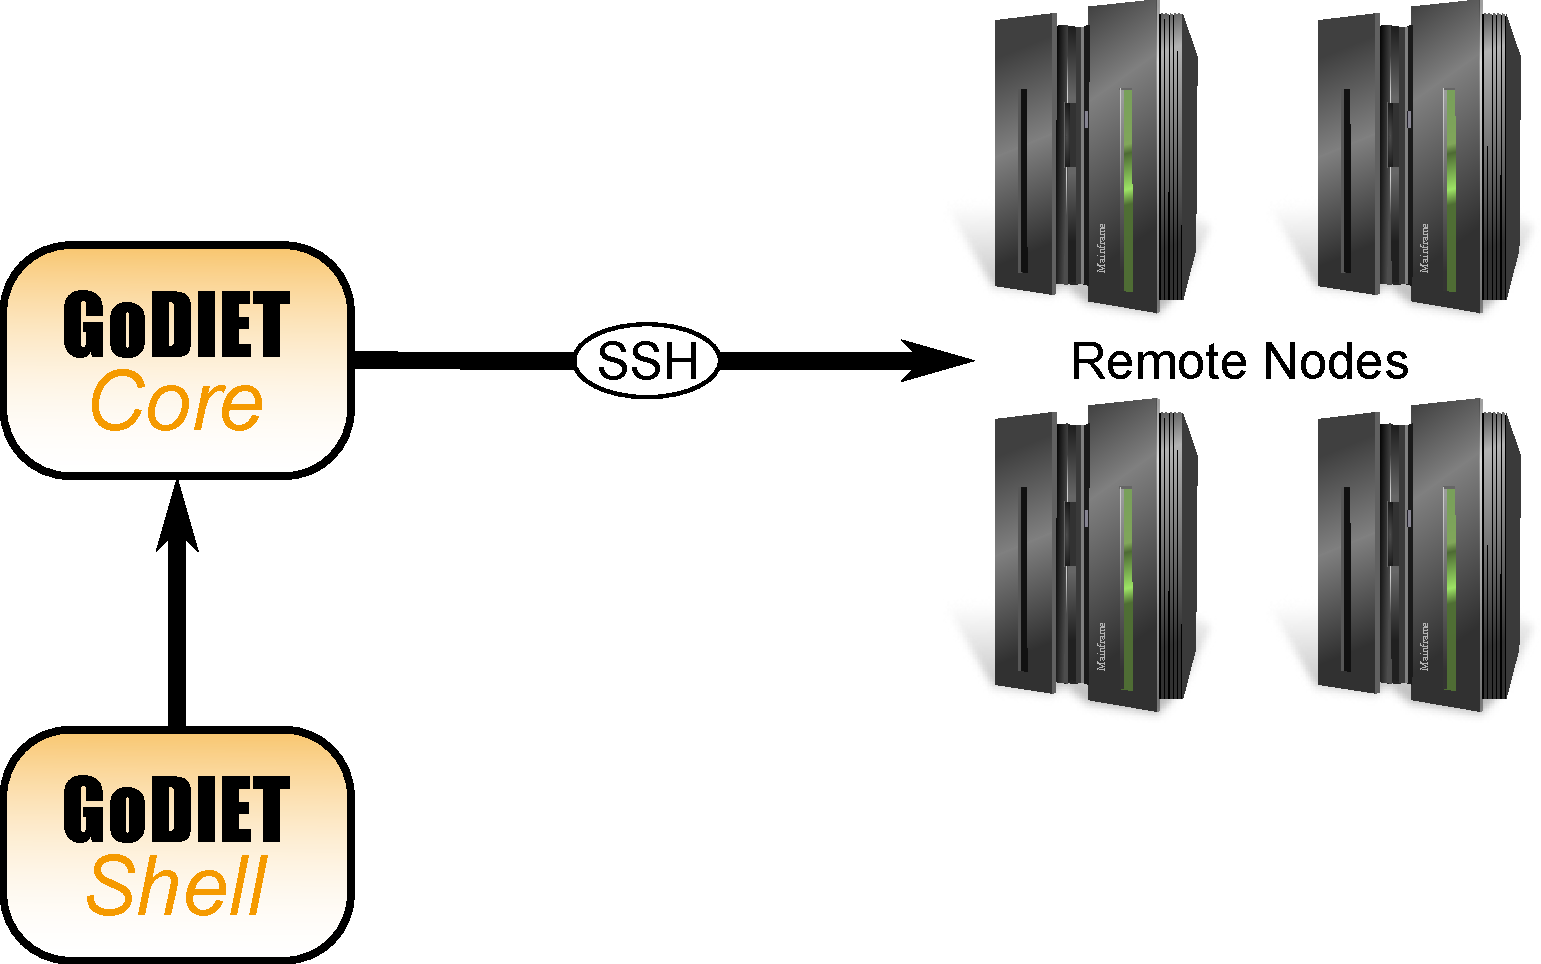
\includegraphics[width=10cm]{fig/schemaPhilippe}
  \caption{Design principle of \godiet.\label{fig:GODIETDesign}}
\end{figure}


\subsection{Installing \godiet}

\bla\subsubsection{Requirement}

The following operating systems are known to support GoDiet:
\begin{itemize}
    \item Linux: the most recent distributions are likely to work;
    \item Mac OS X 10.4 or later.
\end{itemize}

You need to have Sun Java 6 or OpenJDK6 installed.
Download \godiet core and shell on the project's website\footnote{http://graal.ens-lyon.fr/DIET/godiet.html}.
Check that the run.sh script works: it should display something similar to figure~\ref{fig:GODIETShell}.

% This platform must be describe in a XML file based on \textit{Platform.xsd} grammar. You can find an simple file in the example directory 

\subsubsection{Quickstart}
\bla The steps for people in a hurry:
\begin{itemize}
\bla \item running the server : execute run-server.sh
\bla \item running the client : execute run-client.sh
\item create your \godiet configuration file in \verb+${HOME}/.godiet/configuration.xml+~\ref{GODIETConfiguration}. It contains information for remote connection;
\item create your infrastructure description file~\ref{GODIETInfrastructureDescription}. It describes your compute nodes, gateways and storage nodes;
\item create your \diet platform description file~\ref{GODIETPlatform}. It describes all the \diet elements (agents and SeDs) that you want to deploy and manage;
\item run the \godiet shell~\ref{GODIET}.
\end{itemize}
And that's it!


\bla \subsubsection{\godiet server setup}

distribution.layout
RMI configuration
run-server.sh read configuration.xml\label{GODIETConfiguration}


\bla \subsubsection{\godiet client setup}

distribution.layout
RMI configuration
run-client.sh


\subsection{\bla Running Diet}

Before using \godiet, you need to create three files: one to describe \godiet's configuration, one to describe your infrastructure and one that contains your \diet platform's description.
These files use an XML-format and conform to the Configuration.xsd, Infrastructure.xsd and Diet.xsd grammar files (provide with \godiet), repectively.
Sample files are provided in the \verb+examples+ directory. 

\subsubsection{Configuration.xml}
\label{GODIETConfiguration}

\bla Ce fichier regroupe les informations indispensables pour que le serveur puisse se connecter et executer les applications sur les machines distantes.
This file aggregates information about the local node from where \godiet was launched. It also contains information about user authentication.
By default, \godiet looks in the \verb+${HOME}/.godiet/configuration.xml+ directory.

\vspace{1cm}
The mains elements are:
\begin{itemize}
\item \textbf{localNode}: the name of the node on which \godiet was launched. This name must be present in the infrastructure description file;
\item \textbf{localScratch}: the working directory where \godiet stores its temporary files;
\item \textbf{keys}: the paths of your private ssh keys, which are loaded at \godiet's startup. You can give the public key's path, too. \godiet tries to load a file with the same name as the private key and ending with \verb+.pub+. See the \verb+ssh initkeys+ command~\ref{GODIETSSHCommand} to initialize passwords if your keys are encrypted (i.e. need a passphrase).
\end{itemize}

\vspace{1cm}
General layout of the configuration description (some parts are omitted):
\begin{verbatim}
<godiet:configuration localNode="local" schema="Configuration.xsd">

  <localscratch dir="/tmp/scratch_godiet" />
  <user>
     <ssh>
       <key path="/home/.ssh/id_dsa"/>
       <key path="/home/.ssh/admin_cluster2"/>
     </ssh>
  </user>
</godiet:configuration>
\end{verbatim}

\subsubsection{Infrastructure.xml}
\label{GODIETInfrastructureDescription}

\godiet needs to have the description of the infrastructure on which \diet will be running. 

\vspace{1cm}
You can find the full list of options in the \verb+Infrastructure.xsd+ grammar file. You can also look in the \verb+examples+ directory.

The fields are:

\paragraph{Domain:} aggregates a set of infrastructure elements (nodes, gateways, storage) which are able to communicate with \diet's exchange protocol (i.e., CORBA). Typically, elements separated by a firewall and/or a router must be described in separate domains;
\paragraph{Node:} describe a computing node where agents or SeDs will be running. It could be either a physical or virtual machine;

\paragraph{Link:} defines a directional link par lequel les communications SSH sont possibles. Il existe deux types de liens
\begin{itemize}
 \item Entre un domaine et une machine : typiquement des machines derrière un nat (en violet sur la figure).
 \item Entre deux machines : la source est un routeur.
\end{itemize}

\vspace{1cm}

General layout of the infrastructure description (details are omitted):
\begin{verbatim}
<godiet:infrastructure schema="Infrastructure.xsd">
  <domain id="idDomain1"/>
  <domain id="idDomain2"/>
  ..
  <node id="idNode">
    <ssh id="idInterface" domain="idDomainRef" login="login" 
       server="ip/hostname" port="2022" />
    <scratch dir="/tmp/scratch_runtime/" />
    <ssh id="idInterface" domain="idDomainRef" login="login"
       server="ip/hostname" />
    <scratch dir="/tmp/scratch_runtime/" />
  </node>

  ..
  <link fromDomain="DomainSysferaLB" to="graal" accessref="graalinterface1"/>
  <link from="graal" to="testbedVM" accessref="testbedVMinterface1" />
  ..

</godiet:infrastructure>
\end{verbatim}


\begin{figure}[h]
  \centering
  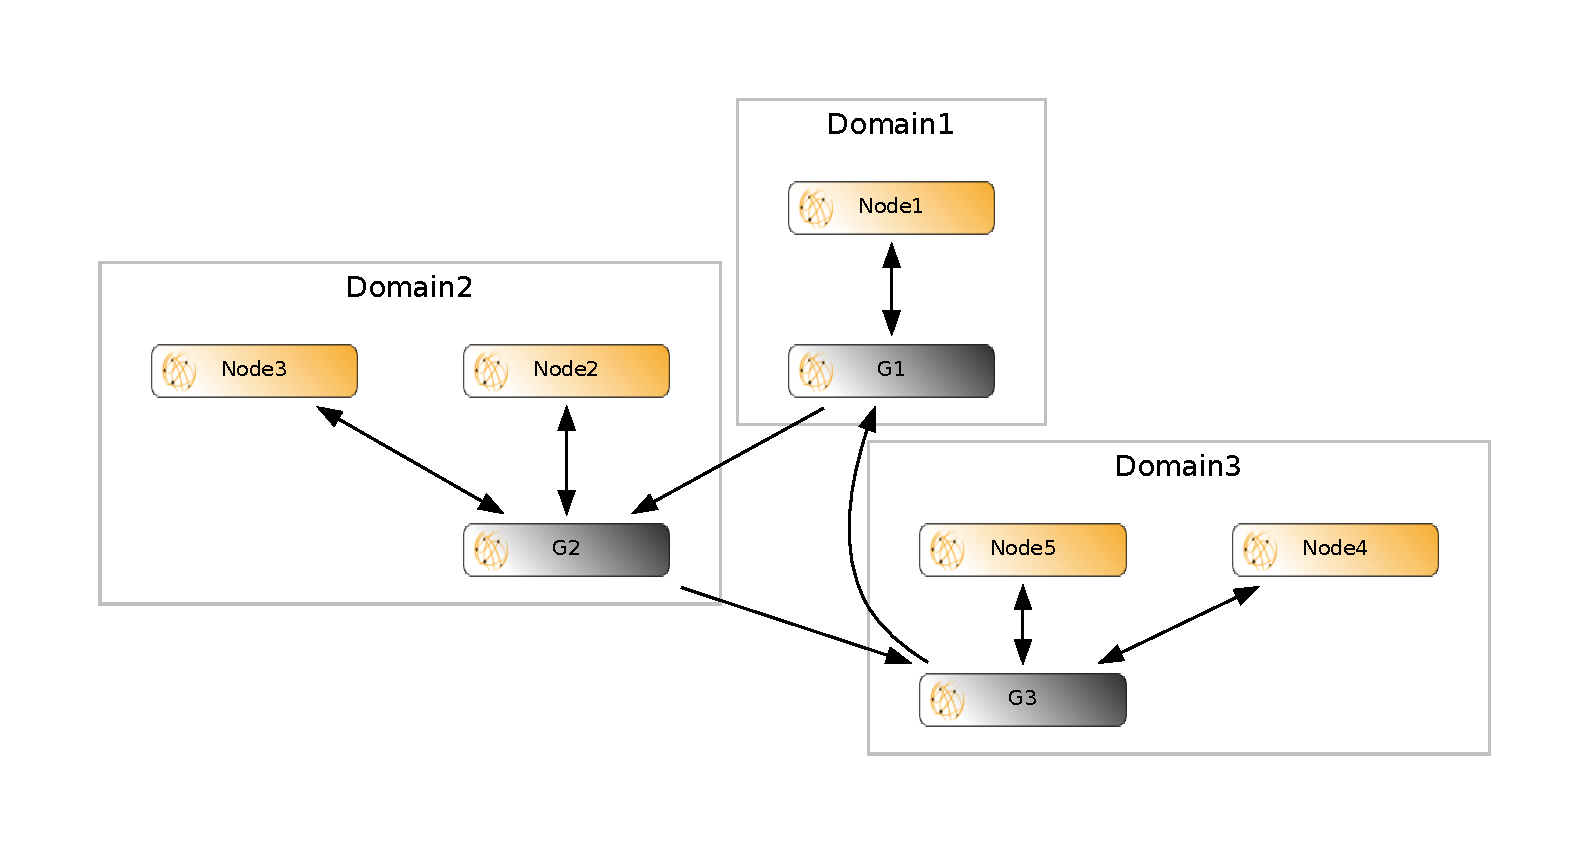
\includegraphics[width=15cm]{fig/godiet-infrastructure}
  \caption{Example of the representation of a three-domain infrastructure.\label{fig:GODIETInfrastructure}}
\end{figure}

\subsubsection{Platform.xml}
\label{GODIETPlatform}

A \godiet user can describe the desired deployment in an XML file including all the external services needed (\eg omniNames and LogService). The desired hierarchical organization of agents and servers is expressed directly using the hierarchical organization of XML. 


The most important fields are:
\begin{itemize}
\item \textbf{dietServices}: lists your \diet services, such as omniNames and LogCentral;
\item \textbf{dietArchitecture}: lists your \diet hierarchy, with all your agents and SeDs. 
\end{itemize}

\vspace{1cm}

General layout of the \diet platform description (details are omitted):


\begin{verbatim}
<godiet:dietPlatform schema="Diet.xsd">
   <services>

    <omniNames id="omniNames1" domain="DomainId1">
	<config server="refIdNode"/>
    </omniNames>
    <omniNames id="omniNames1" domain="DomainId2">
	<config server="refIdNode"/>
    </omniNames>
    <!-- Inter-connect Domain1 and Domain2 -->
    <forwarders>
        <client id="client1" type="CLIENT">
            <config server="refIdNode" />
        </client>
        <server id="server1" type="SERVER">
            <config server="refIdNode" />
        </server>
  <services>


  <hierarchy>
    <ma id="ma1">
 	<config server="refIdNode"/>
	<la id="la1" server="refIdNode">
   	  <config server="refIdNode"/>          
   	  ..
          <sed id="sed1">
	    <config server="refIdNode"/>
	    <file id="sed1_config">
	      <template name="sed_template.config" />
	    </file>
	    <binary name="dmat_manips_server">
	      <commandLine>
	        <parameter string="${this.configurationFiles.sed1_config.absolutePath}" />
	        <parameter string="T" />
	      </commandLine>
	    </binary>
	  </sed>
          ..
       </la>
       ...
     </ma>
     <ma id="ma2" server="refIdNode3">..</ma>
  </hierarchy>

</godiet:dietPlatform>
\end{verbatim}


\subsection{Godiet shell}
\label{GODIETShell}

\godiet shell is the interface to manage and monitor your \diet platform. It includes features such as syntax highlighting, command completion and command history.
To use it, simply execute the script run.sh. You will obtain a prompt like in figure~\ref{fig:GODIETShell}

\begin{figure}[h]
  \centering
  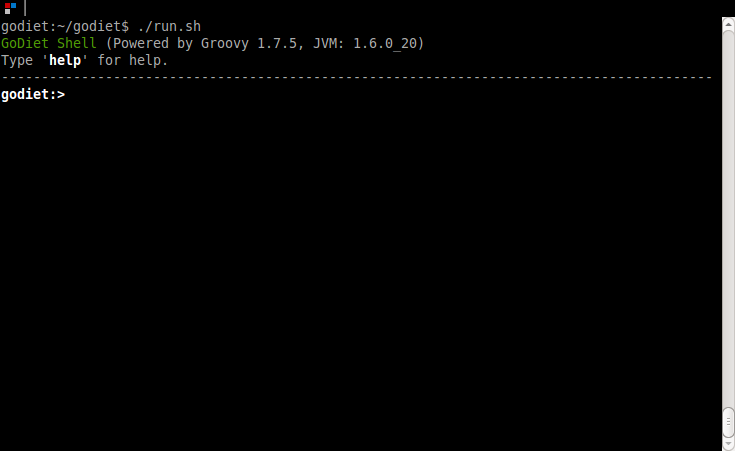
\includegraphics[width=12cm]{fig/1-startup}
  \caption{\godiet shell prompt.\label{fig:GODIETShell}}
\end{figure} 

\subsubsection{The help command}

Displays the help message. By default, lists all the commands and short information about them. It gives contextual help when followed by a command name.

\begin{itemize}
  \item \textbf{command}: gives help on the command.
\end{itemize}

\begin{figure}[h]
  \centering
  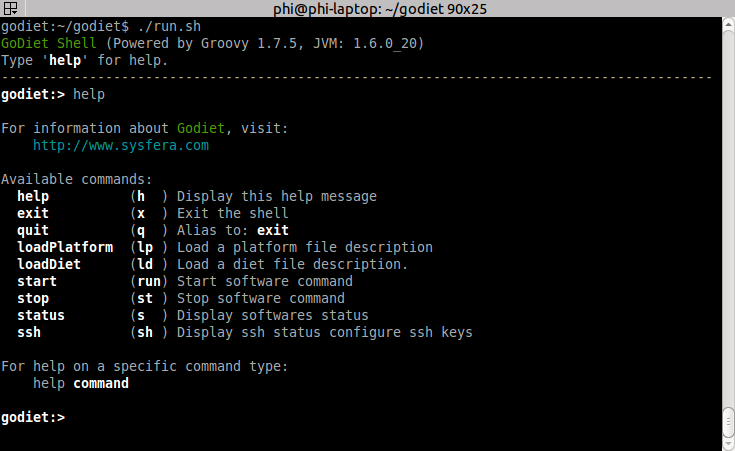
\includegraphics[width=12cm]{fig/2-helpcommand}
  \caption{The help command.\label{fig:GODIETHelp}}
\end{figure}

\subsubsection{The ssh command}
\label{GODIETSSHCommand}

The \verb+ssh+ command takes the following arguments:

\begin{itemize}
\item \textbf{initpasswords}: to intialize the SSH key's passphrase loaded from the configuration file;
\item \textbf{addkey}: to register a new key;
\item \textbf{modifykey n}: to modify a key that has already been registred;
\item \textbf{status}: to display the key's status. Could be PASSWORDNOTSET, PRIVATEKEYERROR, PUBKEYERROR or LOADED.
\end{itemize}

\subsubsection{The loadInfrastructure command}
Loads an infrastructure description file~\ref{GODIETInfrastructureDescription}.

\begin{itemize}
  \item \textbf{filename}: loads an infrastructure from the specified XML file.
\end{itemize}

\subsubsection{The loadDiet command}
Loads the \diet platform description~\ref{GODIETPlatform}. When the loading is complete, \godiet automatically computes and creates all the \diet forwarders needed. These \diet forwarders are mandatory when your platform is deployed on several domains. For more details, please refer to the \diet documentation.

\begin{itemize}
  \item \textbf{filename}: loads a \diet platform from the specified XML file.
\end{itemize}

\subsubsection{The start \& stop commands}
\label{GODIETCommandStartStop}

The \verb+start+ and \verb+stop+ commands both take the same arguments:
\begin{itemize}
 \item \textbf{software} \emph{name}: starts/stops software \emph{name}.
 \item \textbf{services}: starts/stops all services;
 \item \textbf{agents}: starts/stops all agents;
 \item \textbf{seds}: starts/stops all seds;
 \item \textbf{all}: starts/stops all software components;
\end{itemize}

\subsubsection{The status command}

The command displays the status of the \diet platform's software components. It takes the following arguments:
\begin{itemize}
\item \textbf{ma}: displays the status of the master agents;
\item \textbf{la}: displays the status of the local agents;
\item \textbf{seds}: displays the status of the server daemons;
\item \textbf{all}: displays the status of all the managed software components.
\end{itemize}
\vspace{1cm}

%TODO bouger ca dans une section dediee au modele
The \verb+status+ command displays the software components managed by \godiet as a table. Figure~\ref{fig:GODIETStatus} shows an output exemple of this command's execution.
The information is:
\begin{itemize}
\item \textbf{Label}: the name of the component, as described in the \diet platform description;
\item \textbf{Status}: the status of the component;
\item \textbf{Since}: the date since when the component has been in this status;
\item \textbf{Plugged}: the infrastructure resource it is or will be running on (depending on its state);
\item \textbf{Cause}: an information message, in case of error.
\end{itemize} 

\vspace{1cm}
The possible states of a component are:
\begin{itemize}
 \item \textbf{Incubate}: the component is correctly loaded in \godiet;
 \item \textbf{Ready}: the configuration files are created in the local scratch directory and the component is ready to start;
 \item \textbf{Up}: the component is running. Its state is periodically checked;
 \item \textbf{Down}: the componenent is down. Typically, if the \godiet user has used the \verb+stop+ command on this component;
 \item \textbf{Error}: appears when the component is not running (unable to launch or crashed) or if it is unreacheable. The cause is displayed in the Cause row of the information table.  
\end{itemize}

\begin{figure}[h]
  \centering
  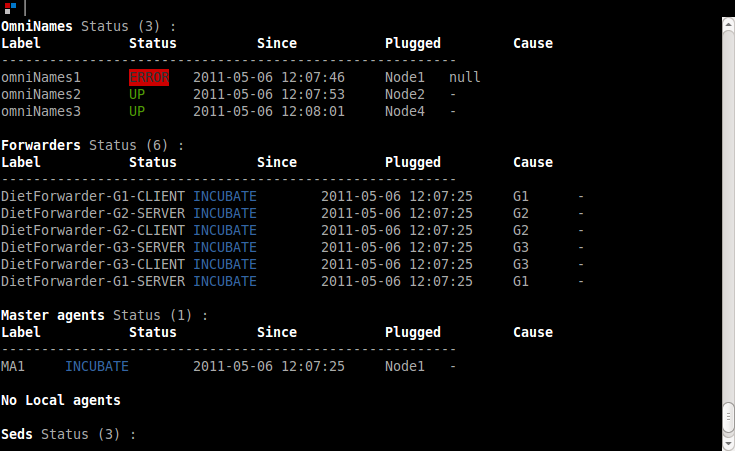
\includegraphics[width=12cm]{fig/6-StatusWithErrUpIncubate}
  \caption{The status command.\label{fig:GODIETStatus}}
\end{figure}

% \subsubsection{Debugging \& Gestion des erreurs}
% parler des fichiers de log et des messages d'erreurs.
